%\documentclass[
  bibliography=totoc,     % Literatur im Inhaltsverzeichnis
  captions=tableheading,  % Tabellenüberschriften
  titlepage=firstiscover, % Titelseite ist Deckblatt
]{scrartcl}

% Paket float verbessern
\usepackage{scrhack}

% Warnung, falls nochmal kompiliert werden muss
\usepackage[aux]{rerunfilecheck}

% unverzichtbare Mathe-Befehle
\usepackage{amsmath}
% viele Mathe-Symbole
\usepackage{amssymb}
% Erweiterungen für amsmath
\usepackage{mathtools}

% Fonteinstellungen
\usepackage{fontspec}
% Latin Modern Fonts werden automatisch geladen
% Alternativ zum Beispiel:
%\setromanfont{Libertinus Serif}
%\setsansfont{Libertinus Sans}
%\setmonofont{Libertinus Mono}

% Wenn man andere Schriftarten gesetzt hat,
% sollte man das Seiten-Layout neu berechnen lassen
\recalctypearea{}

% deutsche Spracheinstellungen
\usepackage[ngerman]{babel}


\usepackage[
  math-style=ISO,    % ┐
  bold-style=ISO,    % │
  sans-style=italic, % │ ISO-Standard folgen
  nabla=upright,     % │
  partial=upright,   % │
  mathrm=sym,        % ┘
  warnings-off={           % ┐
    mathtools-colon,       % │ unnötige Warnungen ausschalten
    mathtools-overbracket, % │
  },                       % ┘
]{unicode-math}

% traditionelle Fonts für Mathematik
\setmathfont{Latin Modern Math}
% Alternativ zum Beispiel:
%\setmathfont{Libertinus Math}

\setmathfont{XITS Math}[range={scr, bfscr}]
\setmathfont{XITS Math}[range={cal, bfcal}, StylisticSet=1]

% Zahlen und Einheiten
\usepackage[
  locale=DE,                   % deutsche Einstellungen
  separate-uncertainty=true,   % immer Unsicherheit mit \pm
  per-mode=symbol-or-fraction, % / in inline math, fraction in display math
]{siunitx}

% chemische Formeln
\usepackage[
  version=4,
  math-greek=default, % ┐ mit unicode-math zusammenarbeiten
  text-greek=default, % ┘
]{mhchem}

% richtige Anführungszeichen
\usepackage[autostyle]{csquotes}

% schöne Brüche im Text
\usepackage{xfrac}

% Standardplatzierung für Floats einstellen
\usepackage{float}
\floatplacement{figure}{htbp}
\floatplacement{table}{htbp}

% Floats innerhalb einer Section halten
\usepackage[
  section, % Floats innerhalb der Section halten
  below,   % unterhalb der Section aber auf der selben Seite ist ok
]{placeins}

% Seite drehen für breite Tabellen: landscape Umgebung
\usepackage{pdflscape}

% Captions schöner machen.
\usepackage[
  labelfont=bf,        % Tabelle x: Abbildung y: ist jetzt fett
  font=small,          % Schrift etwas kleiner als Dokument
  width=0.9\textwidth, % maximale Breite einer Caption schmaler
]{caption}
% subfigure, subtable, subref
\usepackage{subcaption}

% Grafiken können eingebunden werden
\usepackage{graphicx}

% schöne Tabellen
\usepackage{tabularray}
\UseTblrLibrary{booktabs, siunitx}

% Verbesserungen am Schriftbild
\usepackage{microtype}

% Literaturverzeichnis
\usepackage[
  backend=biber,
]{biblatex}
% Quellendatenbank
\addbibresource{lit.bib}
\addbibresource{programme.bib}

% Hyperlinks im Dokument
\usepackage[
  german,
  unicode,        % Unicode in PDF-Attributen erlauben
  pdfusetitle,    % Titel, Autoren und Datum als PDF-Attribute
  pdfcreator={},  % ┐ PDF-Attribute säubern
  pdfproducer={}, % ┘
]{hyperref}
% erweiterte Bookmarks im PDF
\usepackage{bookmark}

% Trennung von Wörtern mit Strichen
\usepackage[shortcuts]{extdash}

\author{%
  Vincent Wirsdörfer\\%
  \href{mailto:vincent.wirsdoerfer@udo.edu}{authorA@udo.edu}%
  \and%
  Joris Daus\\%
  \href{mailto:joris.daus@udo.edu}{authorB@udo.edu}%
}
\publishers{TU Dortmund – Fakultät Physik}


%\begin{document}
\section{Zielsetzung}
\label{sec:Theorie}

\section{Theorie}

Das Ziel des im folgend protokollierten Versuchs besteht in der Bestimmung der effektiven Masse der Leitungselektronen in 
n-dotiertem Galliumarsenid mittels des Faraday-Effekts. 

\subsection{Bandstruktur von Festkörpern}

\noindent Eine Möglichkeit um die Struktur von Festkörpern genauer zu beschreiben ist das sogenannte \textit{Bandstrukturmodell}. Betrachtet man das 
freie Elektronengas, so ergibt sich für die Elektronen im Festkörper eine quadratische Dispersionsrelation:

\begin{equation}
    E(k) = \frac{\hbar²{}k²}{2m}
\end{equation}

\noindent Hierbei steht $\hbar$ für das reduzierte Planck'sche Wirkungsquantum, $k$ für die Wellenzahl und $m$ für die Masse des Elektrons.
Wird nun zusätzlich die Anwesenheit eines perioden Gitterpotentials, ausgelöst durch positive Ionenrümpfe, betrachtet, so ergeben sich verbotene
elektronische Zustände. Jene Energieintervalle, dessen Besetzung erlaubt sind, werden als \textit{Bänder} bezeichnet. Andere Zustände hingegen, welche
energetisch verboten sind, werden als \textit{Bandlücke} beschrieben. Um einen Eindruck zu gewinnen, wie sich das Bändermodell für spezifische
Elektronenkonfigurationen konkretisiert, ist im Folgenden die Bandstruktur von Magnesium abgebildet. 

\begin{figure}[H]
    \centering
    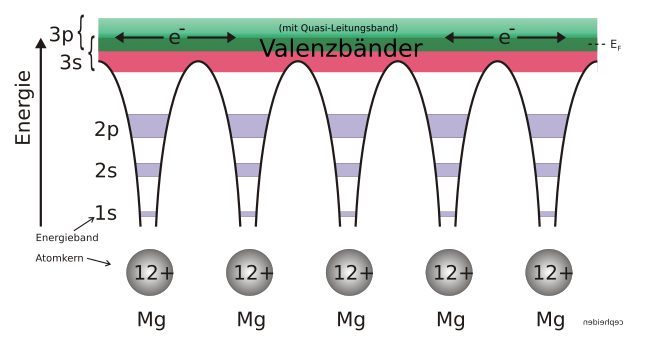
\includegraphics[width=0.7\textwidth]{content/BandstrukturMagn.png}
    \caption{Bandstruktur von Magnesium \cite{Magnesium}.}
    \label{fig:Magnesium}
\end{figure}

\noindent Besonders entscheidend um verschiedene Materialien bzw. Atome zu klassifizieren ist das \textit{Valenz-} und \textit{Leitungsband}. Die Bestzung 
oder Nicht-Besetzung dieser Bänder gibt Aufschluss über die elektrische Leitfähigkeit der betrachteten Materialien und wird maßgeblich von der 
\textit{Fermi-Energie} sowie der Größe der \text{Bandlücke} zwischen ihnen beeinflusst. \\

\noindent Bei \textit{Metallen} liegt die Fermi-Energie im Leitungsband und aufgrund der elektronischen Struktur metallischer Stoffe ist der Übergang beider 
Bänder fließend. Die damit verbundene makroskopische Besetzung des Leitungsbandes führt zu einer höheren elektrischen Leitfähigkeit von Metallen.
Im Gegensatz dazu liegt bei \textit{Isolatoren} eine besonders große Bandlücke vor, was die Besetzung des Leitungsbandes ohne starke äußere Anregung verbietet.
Dies erklärt die geringe elektrische Leitfähigkeit von Isolatoren. Die Bandstruktur von \textit{Halbleitern} ist grundsätzlich nicht einfach von jener der 
Isolatoren zu unterscheiden. Auch hier liegt die Fermi-Energie unterhalb des Leitungsbandes, jedoch ist die Bandlücke in der Regel geringer, was neue 
Möglichkeiten zur Veränderung elektronischer Eigenschaften bietet. Eine Option ist die sogenannte \textit{Dotierung}, welche jedoch im Späteren 
näher erklärt wird. Die folgende Abbildung zeigt, wie sich die verschiedenen Material-Spezifikationen in der Bandstruktur unterscheiden. \\

\begin{figure}[H]
    \centering
    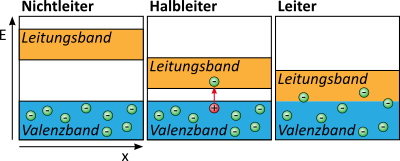
\includegraphics[width=0.7\textwidth]{content/MetIsoHalb.png}
    \caption{Bandstruktur von Isolatoren, Halbleitern und Metallen \cite{Bandstrukturen}.}
    \label{fig:MetIsoHalb}
\end{figure}

\subsection{Dotierung}

\noindent Unter Dotierung versteht man in der Halbleitertechnik die bewusste Verunreinigung von Materialien zur Veränderung
der elektronischen Eigenschaften des Ausgangsmaterials. Die in diesem Experiment verwendete Methode der \textit{n-Dotierung}
bezeichnet das Einfügen von Fremdatomen in das Ausgangsmaterial, welche jeweils über ein zusätzliches Valenzelektron verfügen. 
Die dadurch vorhandenen Elektronen sind nicht statisch an das periodische Gitterpotential gebunden, sondern können sich \enquote{frei} 
durch das Material bewegen. Energetisch liegen die freien Elektronen leicht unter dem Leitungsband.

\begin{figure}[H]
    \centering
    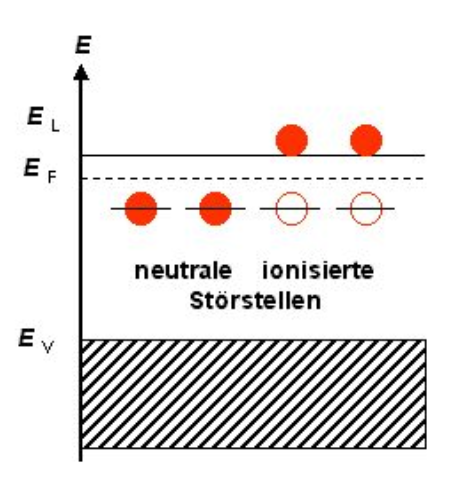
\includegraphics[width=0.4\textwidth]{content/nDot.png}
    \caption{Energetisches Niveau von Donatoren \cite{nDotierung}.}
    \label{fig:nDot}
\end{figure}

\noindent Die effektive Bandlücke zwischen den freien Elektronen und dem Leitungsband ist wesentlich kleiner als die Bandlücke 
zwischen Valenz- und Leitungsband, welche bei üblichen Halbleitermaterialien im Bereich von \qty{1.4}{\electronvolt} liegt. Temperaturen 
in der Nähe von \qty{300}{\kelvin} (Raumtemperatur) können ausreichen, um diese Elektronen in das Leitungsband anzuregen. 
Auf diese Art und Weise kann die elektrische Leitfähigkeit von Halbleitermaterialien signifikant gesteigert werden. 

\subsection{Effektive Masse und Faraday-Effekt}

\noindent Die effektive Masse beschreibt die Wirkung des periodischen Gitterpotentials auf die Masse der Elektronen im Material.
In anisotropen optischen Materialien lässt sich der Tensor der effektiven Masse über die folgende Formel berechnen:

\begin{equation}
    (m^{\ast})_{\text{ij}} = \hbar²\biggl(\frac{\partial²E(\vec{k})}{\partial{}k_{\text{i}}\partial{}k_{\text{j}}}\biggr)^{-1}
    \label{eqn:meff}
\end{equation}

\noindent Wie bereits erläutert, soll in diesem Versuch die effektive Masse der Leitungselektronen von n-dotiertem Galliumarsenid bestimmt 
werden. Dies soll mithilfe des sogenannten \textit{Faraday-Effekts} geschehen. Der Faraday-Effekt beschreibt die Rotation der 
Polarisationsebene von linear polarisiertem Licht in einem Medium, welches von einem parallel zur Ausbreitungsrichtung der Welle gercihteten 
Magnetfeld durchsetzt ist. Dies lässt sich phänomenologisch folgendermaßen erklären: \\

\noindent Das Magnetfeld verändert die Beweglichkeit geladener Teilchen im Medium und bewirkt somit unterschiedliche optische Brechungsindizes
im Material. Eine linear polarisierte Welle lässt sich als Überlagerung einer links- und einer rechtszirkular polarisierten Welle schreiben. 
Durch die anisotropen Brechungsindizes unterscheiden sich nun jedoch die \textit{Phasengeschwindigkeiten} der zirkular polarisierten Wellen, 
was zu einer Phasendifferenz führt. Nach Austritt aus dem Medium hat sich effektiv die Polarisationsebene um einen Winkel $\theta$ gedreht. 
Die folgende Abbildung soll den Effekt skizzenhaft darstellen:

\begin{figure}[H]
    \centering
    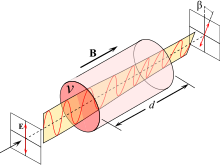
\includegraphics[width=0.4\textwidth]{content/Faraday.png}
    \caption{Faraday-Effekt in einem axial durchsetzten Magnetfeld \cite{Faraday}.}
    \label{fig:Faraday}
\end{figure}

\noindent In einem Kristallgitter verhalten sich die Elektronen nicht wie im Vakuum. Ihre Bewegung wird durch die periodische Potentialstruktur
des Gitters beeinflusst und lässt sich über die effektive Masse $m^{\ast}$ quantifiziert. Je größer die effektive Masse, desto träger 
ihre Reaktion auf extern wirkende Kräfte wie zum Beispiel jene eines magnetischen Feldes. Dies vermindert den Faraday-Effekt und bewirkt 
eine kleinere Winkeländerung als bei einer kleineren effektiven Masse. So lässt sich die Proportionalität

\begin{equation}
    \theta \propto \frac{1}{m^{\ast²}}
\end{equation}

\noindent gut nachvollziehen. Die zentrale Gleichung der Auswertung baut auf diesem Verhältnis auf und lautet

\begin{equation}
    \theta_\text{frei} = \frac{e_0^3}{8 \pi ^2 \varepsilon_0c^3} \frac{NB}{n} \lambda ^2
    \label{eqn:Winkel_frei}
\end{equation}

\noindent Hierbei bezeichnet $\theta_\text{frei}$ den Faraday-Rotationswinkel normiert auf die Probenlänge, $e_0$ die Elementarladung, $N$ die Donatorenkonzentration,
$B$ das maximale Magnetfeld um die Probe, $\varepsilon_0$ die Influenzkonstante, $c$ die Lichtgeschwindigkeit, $n$ den 
Brechungsindex und $m^{\ast}$ die effektive Masse.

\section{Fehlerrechnung}
\label{sec:Fehlerrechnung}

Alle im Protokoll vermerkten Mittelwerte lassen sich über die folgende Formel berechnen:

\begin{equation}
\label{eqn:Mittelwert}
    \bar{x} = \frac{1}{N}\sum_{i=1}^N x_i
\end{equation}

\noindent Zudem lässt sich der dazugehörige Fehler des Mittelwerts wie folgt berechnen:

\begin{equation}
\label{eqn:Mittelwertfehler}
    \increment \bar{x} = \sqrt{\frac{1}{N\left(N-1\right)}\sum_{i=1}^N \left(x_i - \bar{x}\right)²}
\end{equation}

\noindent Entsteht ein neuer Fehler durch bereits fehlerbehaftete Größen, so wird die Gauß'sche Fehlerfortpflanzung angewendet:

\begin{equation}
\label{eqn:Fehlerfortpflanzung}
    \increment f = \sqrt{\sum_{i=1}^N \left(\frac{\partial f}{\partial x_i}\right)²\cdot\left(\increment x_i\right)²}
\end{equation}

%\end{document}